\documentclass[preprint,12pt]{elsarticle}

\usepackage{amsmath,amssymb,amsthm}
\usepackage{graphicx}
\usepackage{booktabs}
\usepackage{algorithm}
\usepackage{algpseudocode}
\usepackage[hidelinks]{hyperref}
\usepackage{xcolor}

\newtheorem{proposition}{Proposition}
\newtheorem{definition}{Definition}
\newtheorem{remark}{Remark}

\journal{Chaos, Solitons \& Fractals}

\begin{document}

\begin{frontmatter}

\title{Selective Chaos Control: Dimension-wise Lyapunov Analysis and Minimal Intervention for Stable yet Creative Large Language Model Agents}

\author{Kuhan K\corref{cor1}}
\ead{kuhankailash92@gmail.com}
\cortext[cor1]{Corresponding author.}
\affiliation{organization={Independent Researcher},
             city={Chennai},
             country={India}}

\begin{abstract}
Large language model (LLM) agents generate outputs by iterating a nonlinear map in a high-dimensional space and show sensitive dependence: a meaning-preserving prompt change, or one early wrong token, can redirect the output. Existing remedies either report a single scalar uncertainty or suppress all variability at once. We treat an agent as a discrete dynamical system observed through semantic output dimensions and propose \emph{Selective Chaos Control} (SCC). SCC (i) estimates a finite-step, Lyapunov-style exponent for every output dimension from a small perturbed-input ensemble, producing a chaos map; (ii) applies Ott--Grebogi--Yorke style minimal intervention only to dimensions whose divergence leaves a target band; (iii) keeps controlled variability in creative dimensions through per-dimension temperature feedback; and (iv) re-anchors multi-step agents at a fraction of their predictability horizon, the agent Lyapunov time. We prove that observed divergence brackets the per-dimension error rate, that factorised consensus has a strictly weaker stability condition than whole-output voting, that the temperature law is stable below a critical gain where it undergoes a period-doubling bifurcation, and that horizon-based checkpointing keeps worst-case deviation below tolerance. Numerical studies on the R\"ossler and Lorenz flows and on synthetic structured-output agents show that the dimension-wise exponent localises errors (AUROC 0.947), that SCC reaches 92.4\% full-output accuracy at 5.6 model calls versus 56.5\% for whole-output self-consistency at 5 calls, and that Lyapunov-time checkpointing raises multi-step success from 79.8\% to 99.8\% at equal cost. We outline extensions to autonomous robots and behavioural time series, and a text-to-SQL evaluation protocol.
\end{abstract}

\begin{keyword}
Chaos control \sep Finite-time Lyapunov exponent \sep Predictability horizon \sep Large language models \sep Autonomous agents \sep Period-doubling bifurcation \sep Selective chaos
\end{keyword}

\end{frontmatter}

%% ===================================================================
\section{Introduction}
\label{sec:intro}

Lorenz's discovery that a three-variable model of convection amplifies a rounding error of $10^{-4}$ into a different forecast~\cite{lorenz1963} established that deterministic rules do not imply long-term predictability. The rate of that amplification, the largest Lyapunov exponent, fixes a predictability horizon beyond which forecasts carry no information; for midlatitude weather this limit is about two weeks~\cite{lorenz1969,zhang2019}. A second insight, due to Ott, Grebogi and Yorke (OGY)~\cite{ott1990}, is that the same sensitivity makes chaotic systems cheap to control: small, well-timed perturbations applied only when the trajectory leaves a target region suffice to stabilise it~\cite{shinbrot1993,boccaletti2000}.

Large language models (LLMs) used as autonomous agents are, mechanically, iterated nonlinear maps on a very high-dimensional state. Each generated token is fed back as input; tool results and earlier steps are appended to the context. Empirical work has documented the expected consequences: meaning-preserving prompt edits shift accuracy by tens of points~\cite{sclar2024,salinas2024}; single tokens act as forking points that redirect the continuation~\cite{bigelow2025}; early hallucinations ``snowball'' into later ones~\cite{zhang2024snowball}; and per-step errors compound over long tasks~\cite{sinha2026}. Recent analyses report quasi-Lyapunov exponents across transformer layers~\cite{li2025quasi}, chaotic signatures in chain-of-thought trajectories~\cite{jaca2026}, period-doubling and chaos in closed LLM feedback loops~\cite{jones2026}, and the amplification of tiny perturbations in multi-LLM committees~\cite{shimao2026}.

Two families of remedies exist. Uncertainty estimators reduce the variability of sampled answers to one number, such as semantic entropy~\cite{kuhn2023,farquhar2024} or sentence-level inconsistency~\cite{manakul2023}, and stability-aware probes flag hallucinations near the boundary between stable and unstable regions~\cite{luan2026}. Variance-reduction methods, such as self-consistency voting~\cite{wang2023sc}, lower temperatures, or verification of every step~\cite{lightman2024}, suppress variability uniformly. Neither family asks \emph{where} in the output the instability lives, and neither distinguishes harmful divergence (a wrong filter in a database query) from useful divergence (an alternative wording or an exploratory plan). The edge-of-chaos literature suggests that some variability is computationally valuable~\cite{bertschinger2004,poole2016,schoenholz2017}; uniform suppression discards it.

This paper imports the two classical ideas, Lyapunov-rate measurement and minimal OGY-type control, into LLM agents, at the level of semantic output dimensions. Its contributions are:
\begin{enumerate}
\item A dynamical-systems formulation of an LLM agent observed through $D$ semantic output dimensions, with a dimension-wise finite-step exponent estimated from a small perturbation ensemble (Section~\ref{sec:model}).
\item Theory: a bracket relating observed divergence to the per-dimension error rate (Proposition~\ref{prop:bracket}); a proof that factorised consensus has a strictly weaker stability condition than whole-output voting (Proposition~\ref{prop:joint}); the stability region and period-doubling bifurcation of a per-dimension temperature feedback law (Proposition~\ref{prop:temp}); and a worst-case deviation bound and optimal allocation for horizon-based checkpointing (Propositions~\ref{prop:horizon} and~\ref{prop:alloc}).
\item The Selective Chaos Control (SCC) architecture, with dimension controllers, a horizon manager and a master controller (Section~\ref{sec:scc}), together with an open implementation.
\item Numerical evidence on canonical chaotic flows and synthetic agents (Section~\ref{sec:numerics}), an evaluation protocol for text-to-SQL agents, and applications to robotics and behavioural time series (Section~\ref{sec:applications}).
\end{enumerate}

%% ===================================================================
\section{Background}
\label{sec:background}

\subsection{Dimension, chaos and predictability}
For autonomous continuous-time flows, the Poincar\'e--Bendixson theorem rules out chaos in the plane: a bounded trajectory of a smooth planar flow approaches a fixed point or a periodic orbit~\cite{strogatz2015,perko2001}. Chaos therefore needs at least three dimensions, as in the R\"ossler~\cite{rossler1976}, Lorenz~\cite{lorenz1963}, Thomas~\cite{thomas1999}, Rucklidge~\cite{rucklidge1992} and Halvorsen~\cite{sprott2010} systems; four or more dimensions admit hyperchaos with several positive exponents~\cite{rossler1979}. The restriction does not apply to discrete-time maps, which can be chaotic in one dimension. LLM agents are discrete maps, so the relevant question for them is not \emph{whether} chaos is admissible but \emph{in which output dimensions} perturbations are amplified.

The largest Lyapunov exponent $\lambda$ measures the mean exponential separation rate of nearby trajectories, $\|\delta(t)\|\approx\|\delta(0)\|e^{\lambda t}$. It can be estimated from data by tracking neighbouring trajectories~\cite{wolf1985,rosenstein1993} or by renormalised tangent dynamics~\cite{benettin1980}; finite-time Lyapunov exponents (FTLE) quantify separation over a finite window~\cite{shadden2005}. An initial error $e_0$ reaches tolerance $\Delta$ after the predictability horizon
\begin{equation}
T_h=\frac{1}{\lambda}\ln\frac{\Delta}{e_0}, \label{eq:horizon}
\end{equation}
so a tenfold improvement in $e_0$ extends $T_h$ only by $\ln 10/\lambda$, which is why the weather horizon resists better observation~\cite{lorenz1969,zhang2019}.

\subsection{Controlling chaos}
A chaotic attractor contains infinitely many unstable periodic orbits. OGY control~\cite{ott1990} waits until the trajectory passes near a chosen orbit and applies the smallest parameter perturbation that places it on the orbit's stable manifold; delayed-feedback control~\cite{pyragas1992} achieves similar effects without a model. Both exploit the fact that intervention is needed only intermittently and in small amounts~\cite{shinbrot1993,boccaletti2000}, a principle used in practice to steer spacecraft along low-energy trajectories~\cite{belbruno1993}. Synchronisation of chaotic systems~\cite{pecora1990} shows that coupling can also remove chaos.

\subsection{LLM uncertainty, sensitivity and agents}
Semantic entropy clusters sampled answers by meaning and computes entropy over clusters~\cite{kuhn2023,farquhar2024}; SelfCheckGPT scores sentences by sample disagreement~\cite{manakul2023}; self-consistency takes a majority over reasoning paths~\cite{wang2023sc}; models can also verbalise confidence~\cite{kadavath2022}; and conformal methods provide coverage guarantees~\cite{quach2024,mohri2024}. Hallucination taxonomies are surveyed in~\cite{huang2025survey}. Activation steering~\cite{zou2023repe,turner2023,li2023iti} shows that LLM internal dynamics can be controlled, and adaptive temperature methods vary randomness token by token using the model's own entropy~\cite{zhu2024adapt,zhang2024edt}. Agentic frameworks interleave reasoning and tool calls~\cite{yao2023react}, add self-reflection~\cite{shinn2023,madaan2023}, tool-based critique~\cite{gou2024critic}, multi-agent debate~\cite{du2024debate} and step-level verification~\cite{lightman2024}; their failure modes are catalogued in~\cite{cemri2025}. Text-to-SQL is a demanding testbed with execution-accuracy benchmarks~\cite{yu2018spider,li2023bird,lei2025spider2} and decomposed or multi-agent pipelines~\cite{pourreza2023,gao2024dail,talaei2024chess,wang2025macsql}.

In this journal, neural networks have been used to forecast chaotic series~\cite{valle2025,crespo2024,pathak2018}, and Lyapunov stability has served as an instability signal for neural classifiers~\cite{pedraza2022}. Table~\ref{tab:gap} positions the present work.

\begin{table}[t]
\centering
\small
\caption{Position of SCC relative to prior work. \checkmark: provided; --: not provided.}
\label{tab:gap}
\resizebox{\textwidth}{!}{%
\begin{tabular}{lcccc}
\toprule
Method family & Per-dimension & Growth rate & Selective control & Horizon schedule \\
\midrule
Semantic entropy, SelfCheckGPT~\cite{farquhar2024,manakul2023} & -- / partial & -- & -- & -- \\
Self-consistency, verify-all~\cite{wang2023sc,lightman2024} & -- & -- & -- (uniform) & -- \\
Quasi-Lyapunov, Lyapunov probes~\cite{li2025quasi,luan2026} & -- & \checkmark & -- & -- \\
Activation steering~\cite{zou2023repe,li2023iti} & -- & -- & -- (always on) & -- \\
Adaptive temperature~\cite{zhu2024adapt,zhang2024edt} & token-level & -- & partial & -- \\
\textbf{SCC (this work)} & \checkmark & \checkmark & \checkmark & \checkmark \\
\bottomrule
\end{tabular}}
\end{table}

%% ===================================================================
\section{LLM agents as dimension-observed dynamical systems}
\label{sec:model}

\subsection{State, map and observation}
Let an agent receive input $x\in\mathcal{X}$ (prompt, context and tool results) and produce an output $y=F(x,\xi;\tau)\in\mathcal{Y}$, where $\xi$ is sampling noise and $\tau$ a temperature. In a multi-step agent the context evolves as $x_{t+1}=G(x_t,y_t)$, so the agent is a discrete-time random dynamical system on $\mathcal{X}$. We do not observe the internal state; we observe the output through a \emph{semantic decomposition}
\begin{equation}
\Pi:\mathcal{Y}\to\mathcal{V}_1\times\cdots\times\mathcal{V}_D,\qquad \Pi(y)=(y_1,\dots,y_D),
\end{equation}
with a bounded metric $\rho_j:\mathcal{V}_j\times\mathcal{V}_j\to[0,1]$ on each component. For a SQL-generating agent, the dimensions are the referenced tables, the projection, the joins, the predicates, the grouping and aggregation, and the ordering and limit; $\rho_j$ is a Jaccard distance on sets of canonicalised clauses. Each dimension also carries a \emph{role}: \emph{precision} (errors are harmful and variation should be suppressed) or \emph{creative} (variation is acceptable or useful, e.g.\ explanatory text, alternative plans, exploration in a robot).

\subsection{Perturbation ensemble and dimension-wise divergence}
Let $\{x^{(k)}\}_{k=1}^{K}$ be meaning-preserving perturbations of $x$ (paraphrases, synonym substitutions, formatting changes, or independent samples), with mean input distance $\varepsilon=\frac{1}{K-1}\sum_{k\ge 2}\rho_{\mathrm{in}}(x,x^{(k)})$. With outputs $y^{(k)}=F(x^{(k)},\xi_k;\tau)$ we define the dimension-wise divergence as the U-statistic
\begin{equation}
d_j=\binom{K}{2}^{-1}\sum_{a<b}\rho_j\!\left(y^{(a)}_j,y^{(b)}_j\right)\in[0,1],
\label{eq:div}
\end{equation}
and the \emph{dimension-wise finite-step exponent}
\begin{equation}
\hat\lambda_j=\ln\frac{\max(d_j,d_{\min})}{\varepsilon},
\label{eq:lam}
\end{equation}
where $d_{\min}>0$ is a resolution floor. $\hat\lambda_j>0$ means that dimension $j$ amplifies input perturbations; $\hat\lambda_j<0$ means it contracts them. In a multi-step agent, $d_j(t)$ is tracked along the trajectory and $\lambda_j$ is the least-squares slope of $\ln d_j(t)$, in the manner of~\cite{rosenstein1993}. The vector $(\hat\lambda_1,\dots,\hat\lambda_D)$ is the \emph{chaos map} of the query.

\begin{remark}
In a smooth flow, a generic perturbation eventually aligns with the leading Lyapunov vector, so all coordinates share the same asymptotic exponent. At finite times, however, coordinates can differ by orders of magnitude (Fig.~\ref{fig:flows}c). Semantic output dimensions of an LLM are moreover produced by largely separate parts of the computation and can be nearly decoupled; dimension-wise finite-step rates are therefore the informative quantity.
\end{remark}

\subsection{Divergence brackets the error rate}
Consider a precision dimension with exact-match metric and $K$ i.i.d.\ samples whose value is correct with probability $1-p$ and otherwise takes wrong value $i$ with probability $q_i$, $\sum_i q_i=p$.

\begin{proposition}[Divergence--error bracket]
\label{prop:bracket}
$\mathbb{E}[d_j]=1-(1-p)^2-\sum_i q_i^2$, hence $2p(1-p)\le\mathbb{E}[d_j]\le 2p-p^2$. For $p\le\tfrac12$ and $\mathbb{E}[d_j]\le\tfrac12$,
\begin{equation}
1-\sqrt{1-\mathbb{E}[d_j]}\;\le\;p\;\le\;\tfrac12\left(1-\sqrt{1-2\,\mathbb{E}[d_j]}\right).
\label{eq:bracket}
\end{equation}
\end{proposition}
\begin{proof}
Two independent samples agree iff both are correct or both take the same wrong value, with probability $(1-p)^2+\sum_i q_i^2$. The U-statistic~\eqref{eq:div} is unbiased for one minus that probability. Since $0\le\sum_i q_i^2\le(\sum_i q_i)^2=p^2$, the stated bounds follow; the lower bound corresponds to a single wrong alternative and the upper to diffuse wrong answers. Inverting the monotone functions $2p(1-p)$ and $2p-p^2$ on $[0,\tfrac12]$ gives~\eqref{eq:bracket}.
\end{proof}
The bracket converts an observable, $d_j$, into an error-rate estimate for each dimension without labels; it is the quantity on which the control law acts.

\subsection{The curse of joint agreement}
Self-consistency~\cite{wang2023sc} votes over \emph{whole} outputs. With independent dimensions, a sample is fully correct with probability $\prod_j(1-p_j)$, which decays exponentially in $D$.

\begin{proposition}[Factorised versus joint consensus]
\label{prop:joint}
Let dimensions be independent with error rates $p_j$, and consider strict-majority voting over $K$ samples. Whole-output voting is consistent ($\Pr[\text{correct}]\to1$ as $K\to\infty$) if $1-\prod_j(1-p_j)<\tfrac12$; factorised voting, a separate vote per dimension, is consistent if $\max_j p_j<\tfrac12$, with
\begin{equation}
\Pr[\text{factorised output wrong}]\le\sum_{j=1}^{D}\exp\!\left(-2K\left(\tfrac12-p_j\right)^2\right).
\label{eq:hoeff}
\end{equation}
Since $1-\prod_j(1-p_j)\ge\max_j p_j$, with equality only if at most one $p_j>0$, the factorised condition is strictly weaker.
\end{proposition}
\begin{proof}
For dimension $j$, the number of correct samples is $\mathrm{Bin}(K,1-p_j)$; by Hoeffding's inequality the probability that it fails to exceed $K/2$ is at most $\exp(-2K(\frac12-p_j)^2)$. A union bound over $j$ gives~\eqref{eq:hoeff}. The whole-output case is the same argument with a single Bernoulli variable of success probability $\prod_j(1-p_j)$. The final inequality holds because $\prod_j(1-p_j)\le 1-p_m$ for every $m$.
\end{proof}
For six dimensions with $p_j=0.15$, factorised voting is consistent while whole-output voting has a fully-correct rate of only $0.377$; plurality voting with diffuse wrong answers is somewhat more forgiving, but the gap persists (Section~\ref{sec:numerics}).

%% ===================================================================
\section{Selective Chaos Control}
\label{sec:scc}

\subsection{Minimal intervention law}
Each precision dimension has a target band $[\theta^{\mathrm{lo}}_j,\theta^{\mathrm{hi}}_j]$, normally $[0,\theta_j]$. In the spirit of OGY control, a dimension controller does nothing while $d_j$ stays inside its band and otherwise applies the cheapest action from an intervention ladder: (a0) none; (a1) factorised consensus, taking the plurality or medoid value of the $K$ samples at no extra cost; (a2) grounding, regenerating only dimension $j$ with targeted context such as schema facts or retrieved records at temperature zero; (a3) verification against an external oracle such as executing a probe query or a physics check; and (a4) escalation to a human. Formally, with action costs $c_0=c_1=0<c_2<c_3<c_4$ and predicted post-action error $\hat p_j(a)$, obtained from~\eqref{eq:bracket} for (a1) and from calibration for (a2)--(a4),
\begin{equation}
a_j^\star=\arg\min_{a}\;c_a\quad\text{s.t.}\quad \hat p_j(a)\le p^{\mathrm{tol}}_j .
\label{eq:ladder}
\end{equation}
The expected cost per query is $K+\sum_j c_2\Pr[d_j>\theta_j]$ (for a2), compared with $1+Dc_2$ for verify-all; savings scale with the fraction of stable dimensions.

\subsection{Selective chaos through temperature feedback}
Creative dimensions should keep their divergence inside a band $[\theta^{\mathrm{lo}}_j,\theta^{\mathrm{hi}}_j]$ with midpoint $d^\star_j$, while precision dimensions are driven toward $d_j\to0$. Each dimension keeps its own temperature $\tau_j$, updated by a log-proportional law
\begin{equation}
u_{n+1}=u_n-\eta\left(g_j\!\left(e^{u_n}\right)-d_j^\star\right),\qquad u=\ln\tau_j,
\label{eq:temp}
\end{equation}
where $g_j(\tau)=\mathbb{E}[d_j\mid\tau]$ is the (unknown, increasing) divergence response of dimension $j$. In practice the controller uses the measured $d_j$ in place of $g_j$. Dimension-specific temperatures are implemented by generating the dimensions in separate calls or with constrained decoding.

\begin{proposition}[Stability and bifurcation of the temperature law]
\label{prop:temp}
Let $g_j$ be $C^1$ and increasing with fixed point $g_j(\tau^\star)=d^\star_j$. The map~\eqref{eq:temp} has the fixed point $u^\star=\ln\tau^\star$ with multiplier $\mu=1-\eta\,\tau^\star g_j'(\tau^\star)$. The fixed point is asymptotically stable iff
\begin{equation}
0<\eta<\eta_c=\frac{2}{\tau^\star g_j'(\tau^\star)},
\label{eq:etac}
\end{equation}
and at $\eta=\eta_c$ the multiplier crosses $-1$, a flip (period-doubling) bifurcation.
\end{proposition}
\begin{proof}
Differentiating the right-hand side of~\eqref{eq:temp} with respect to $u$ gives $1-\eta\,e^{u}g_j'(e^{u})$, which equals $\mu$ at $u^\star$. Linear stability of a one-dimensional map requires $|\mu|<1$, which gives~\eqref{eq:etac}; $\mu=-1$ at $\eta_c$ is the flip condition.
\end{proof}
Proposition~\ref{prop:temp} makes the controller's own nonlinear dynamics explicit: an over-aggressive gain turns the stabiliser into an oscillator, the classical failure mode of high-gain feedback on a nonlinear plant.

\subsection{Agent Lyapunov time and checkpoint scheduling}
In multi-step agents the deviation from a correct trajectory grows approximately as $e(t)=e_0e^{\lambda t}$ between re-anchoring events (verification, grounding, or a reset to a validated state). We call $1/\lambda$ the \emph{agent Lyapunov time} and $T_h$ in~\eqref{eq:horizon} the agent's predictability horizon.

\begin{proposition}[Horizon-based checkpointing]
\label{prop:horizon}
If the growth rate between checkpoints does not exceed $\lambda>0$ and every checkpoint resets the deviation to $e_0$, then checkpointing every $\alpha T_h$ steps, $0<\alpha<1$, guarantees
\begin{equation}
e_{\max}\le e_0\left(\frac{\Delta}{e_0}\right)^{\alpha}<\Delta .
\label{eq:emax}
\end{equation}
\end{proposition}
\begin{proof}
Between checkpoints $e(t)\le e_0\exp(\lambda\alpha T_h)=e_0\exp(\alpha\ln(\Delta/e_0))$.
\end{proof}

\begin{proposition}[Optimal checkpoint allocation]
\label{prop:alloc}
Consider tasks $i=1,\dots,N$ of length $L$ with rates $\lambda_i$ and a common target $e_{\max}\le e^\star$. The minimum total number of checkpoints is $\sum_i L\lambda_i/\ln(e^\star/e_0)$, attained by intervals $\Delta t_i\propto1/\lambda_i$. A single fixed interval must satisfy the fastest task and needs $NL\lambda_{\max}/\ln(e^\star/e_0)$, so the adaptive schedule uses a fraction $\bar\lambda/\lambda_{\max}$ of the fixed schedule's checkpoints.
\end{proposition}
\begin{proof}
Task $i$ meets the target iff $\Delta t_i\le\ln(e^\star/e_0)/\lambda_i$; the number of checkpoints $L/\Delta t_i$ is minimised at equality. A common interval must satisfy the constraint for $\lambda_{\max}$.
\end{proof}
The rate $\lambda$ is unknown in advance, so the horizon manager estimates it online from the deviation series by the least-squares slope of $\ln e(t)$ and sets the interval to $\max\{1,\lfloor\alpha\hat T_h\rfloor\}$.

\subsection{Master controller}
The master controller (Algorithm~\ref{alg:scc}) composes the per-dimension decisions, checks cross-dimension consistency (for example, projected columns must belong to selected tables; a robot's planned path must respect its speed limit), re-routes violating dimensions through the ladder, and reports a global stability index
\begin{equation}
S=1-\frac{\sum_j w_jd_j}{\sum_j w_j}\in[0,1].
\end{equation}

\begin{algorithm}[t]
\caption{Selective Chaos Control for one agent step}
\label{alg:scc}
\begin{algorithmic}[1]
\Require input $x$, ensemble size $K$, decomposition $\Pi$, bands $\{[\theta_j^{\mathrm{lo}},\theta_j^{\mathrm{hi}}]\}$, temperatures $\{\tau_j\}$
\State $\{x^{(k)}\}\gets$ \Call{Perturb}{$x,K$}; $\varepsilon\gets$ mean input distance
\State $y^{(k)}\gets F(x^{(k)},\xi_k;\tau)$ for $k=1..K$; \quad $(y^{(k)}_1,\dots,y^{(k)}_D)\gets\Pi(y^{(k)})$
\For{$j=1..D$}
  \State $d_j\gets$ Eq.~\eqref{eq:div};\quad $\hat\lambda_j\gets\ln(\max(d_j,d_{\min})/\varepsilon)$
  \If{role$_j$ = creative} \State update $\tau_j$ by Eq.~\eqref{eq:temp}; keep one sample
  \ElsIf{$d_j\in[\theta_j^{\mathrm{lo}},\theta_j^{\mathrm{hi}}]$} \State $v_j\gets$ consensus value
  \Else \State $v_j\gets$ cheapest ladder action meeting $p_j^{\mathrm{tol}}$ (Eq.~\eqref{eq:ladder}); update $\tau_j$
  \EndIf
\EndFor
\State repair dimensions that violate cross-dimension constraints
\State \Return composed output $y^\star$, chaos map $(\hat\lambda_j)$, stability index $S$
\end{algorithmic}
\end{algorithm}

%% ===================================================================
\section{Numerical study}
\label{sec:numerics}

All experiments are deterministic given a fixed random seed and run in under a minute on a laptop; the scripts accompany the paper. Experiments E3--E5 use a synthetic agent whose ground truth is known. They test the internal logic of SCC, not the behaviour of any particular LLM; Section~\ref{sec:protocol} gives the empirical protocol.

\subsection{E1: dimension-wise separation in canonical flows}
Twin trajectories of the R\"ossler ($a=b=0.2$, $c=5.7$) and Lorenz ($\sigma=10$, $r=28$, $b=8/3$) systems, separated by $10^{-8}$ in $x$ after a burn-in, were integrated with relative and absolute tolerance $10^{-11}$. Per-coordinate separations, normalised by attractor extent, are shown in Fig.~\ref{fig:flows}. Fitted dimension-wise exponents are $0.903$, $0.885$ and $0.886$ for Lorenz (reference value $\approx0.906$) and $0.060$, $0.060$ and $0.052$ for R\"ossler (reference $\approx0.071$). All coordinates share the asymptotic rate, as theory predicts, but at finite times the R\"ossler $z$-separation differs from the $x$-separation by up to three orders of magnitude (5th--95th percentile of $\log_{10}(d_z/d_x)$: $-3.07$ to $0.45$). A single-snapshot sensor in the wrong coordinate would therefore misjudge the state by a factor of up to $10^3$, which motivates reading every dimension separately.

\begin{figure}[t]
\centering
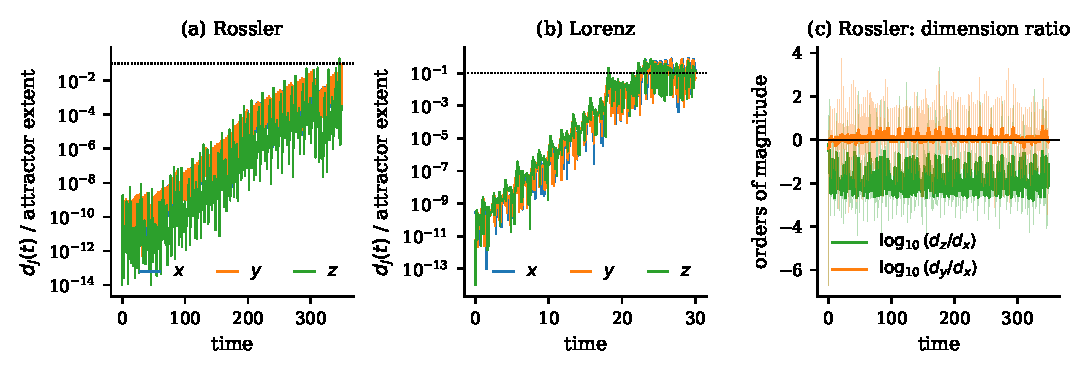
\includegraphics[width=\textwidth]{figures/fig1_dimensionwise_divergence.pdf}
\caption{E1. Per-dimension separation of twin trajectories, normalised by attractor extent, for (a) R\"ossler and (b) Lorenz; the dotted line marks 10\% of the extent. (c) Finite-time ratio of R\"ossler separations: thin lines are raw values and thick lines are running means.}
\label{fig:flows}
\end{figure}

\subsection{E2: divergence--error bracket}
For error rates $p\in[0.01,0.45]$, ensembles of $K=7$ samples were drawn with either one wrong alternative or 50 diffuse alternatives (400 repetitions each). All 60 mean divergences fall inside the bracket of Proposition~\ref{prop:bracket} to within $0.03$ (Fig.~\ref{fig:bracket}); single-alternative points lie on the upper boundary and diffuse points on the lower, as predicted.

\begin{figure}[t]
\centering
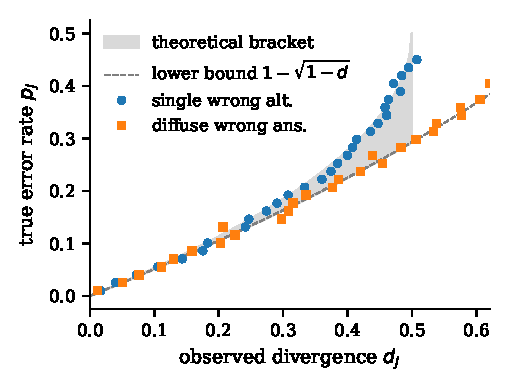
\includegraphics[width=0.55\textwidth]{figures/fig2_divergence_error_bracket.pdf}
\caption{E2. Observed divergence against true error rate with the theoretical bracket of Eq.~\eqref{eq:bracket}.}
\label{fig:bracket}
\end{figure}

\subsection{E3: synthetic structured-output agent}
We simulated 4000 queries with $D=6$ precision dimensions. Latent per-dimension error rates follow a heavy-tailed mixture: $\mathrm{Beta}(0.6,12)$ for most dimensions, with 12\% of dimensions ``hard'' at $p\sim U(0.25,0.65)$, reflecting the common observation that errors concentrate in one component of an output. Sampling at $\tau=0.7$ adds $0.15\tau$ to non-trivial error rates, and wrong values are drawn from eight alternatives. Grounding multiplies a dimension's error rate by $0.25$ at a cost of one call. Five strategies were compared: a single greedy call; whole-output self-consistency ($K=5$); verify-all, with one call plus grounding of all six dimensions; factorised consensus ($K=5$, the SCC ablation without grounding); and SCC ($K=5$, grounding iff $d_j>\theta=0.7$).

\begin{table}[t]
\centering
\caption{E3. Full-output accuracy (all six dimensions correct) and mean model calls per query (4000 synthetic queries).}
\label{tab:e3}
\begin{tabular}{lcc}
\toprule
Strategy & Accuracy & Calls/query \\
\midrule
Single greedy & 0.539 & 1.00 \\
Self-consistency, whole output ($K=5$) & 0.565 & 5.00 \\
Verify-all (ground every dimension) & 0.857 & 7.00 \\
Factorised consensus ($K=5$) & 0.842 & 5.00 \\
\textbf{SCC} ($K=5$, $\theta=0.7$) & \textbf{0.924} & \textbf{5.58} \\
\bottomrule
\end{tabular}
\end{table}

Table~\ref{tab:e3} and Fig.~\ref{fig:agent}a summarise the results. Whole-output self-consistency barely improves on a single call at $K=5$ and needs $K=15$ to reach $0.840$, the curse of joint agreement of Proposition~\ref{prop:joint}. Factorised consensus alone reaches $0.842$ at the same cost. SCC grounds only the $\approx0.58$ dimensions per query flagged as unstable and reaches $0.924$, above verify-all ($0.857$), which spends a grounding call on every dimension and forgoes the consensus available for stable ones. The dimension-wise exponent localises errors with AUROC $0.947$ (Fig.~\ref{fig:agent}b). No consensus value was wrong among the 13{,}473 dimensions with $d_j=0$, and the error rate was $0.11\%$ at $d_j=0.4$ (a single dissenting sample), rising to $32\%$ at $d_j=0.9$. Sweeping $\theta$ traces a front (red line) whose operating point at $\theta\approx0.7$ dominates verify-all.

\begin{figure}[t]
\centering
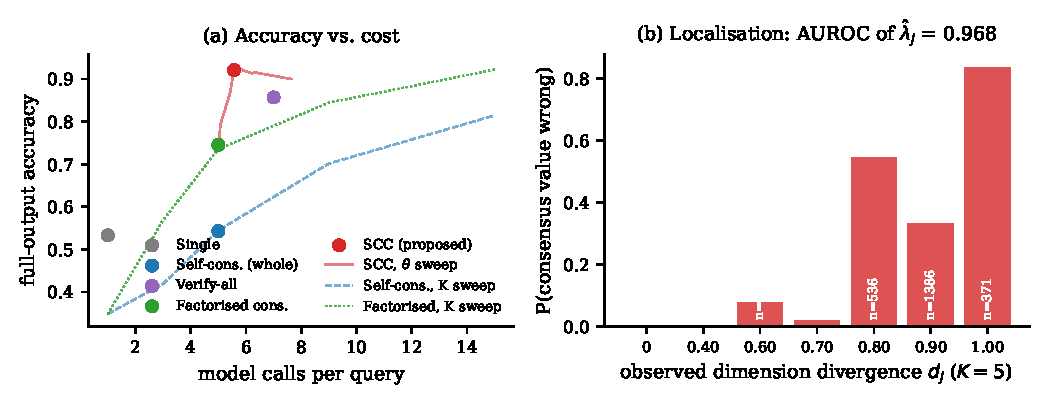
\includegraphics[width=\textwidth]{figures/fig3_agent_accuracy_cost.pdf}
\caption{E3. (a) Accuracy versus cost; lines show threshold and ensemble-size sweeps. (b) Probability that the consensus value of a dimension is wrong, as a function of its observed divergence.}
\label{fig:agent}
\end{figure}

\subsection{E4: Lyapunov-time checkpointing}
We simulated 3000 multi-step agents with $L=40$ steps, $e_0=0.01$, tolerance $\Delta=0.3$, heterogeneous rates $\lambda_i\sim U(0.03,0.7)$ and multiplicative noise $e_{t+1}=e_t\exp(\lambda_i+0.15\,\zeta_t)$ with $\zeta_t\sim\mathcal{N}(0,1)$. A task fails when $e_t>\Delta$. Fixed-interval checkpointing was compared with the adaptive horizon manager, which estimates $\lambda_i$ online and uses interval $\lfloor\alpha\hat T_h\rfloor$ (Fig.~\ref{fig:ckpt}). Without checkpoints, success is $7.8\%$. At equal mean cost the adaptive schedule dominates: $99.8\%$ versus $79.8\%$ at $6.5$ checkpoints per task, and $86.0\%$ versus $68.6\%$ at $4.5$. A fixed schedule needs about $10$ checkpoints per task to exceed $98\%$, consistent with the allocation ratio $\bar\lambda/\lambda_{\max}\approx0.52$ of Proposition~\ref{prop:alloc} plus the overhead of estimating $\lambda$ online.

\begin{figure}[t]
\centering
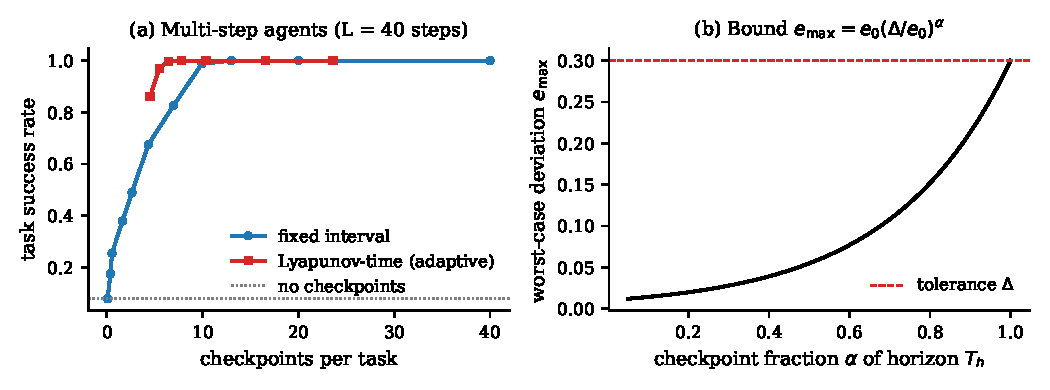
\includegraphics[width=\textwidth]{figures/fig4_lyapunov_time_checkpointing.pdf}
\caption{E4. (a) Task success against checkpoints per task for fixed and Lyapunov-time schedules. (b) Worst-case deviation bound of Proposition~\ref{prop:horizon}.}
\label{fig:ckpt}
\end{figure}

\subsection{E5--E6: selective chaos and controller bifurcation}
Two precision dimensions and one creative dimension (band $[0.2,0.6]$) were controlled by~\eqref{eq:temp} with $\eta=2$ and a saturating response $g_j(\tau)=0.8(1-e^{-a_j\tau})$ plus noise (Fig.~\ref{fig:selective}). The precision temperatures converge to $0.008$ and $0.013$, with divergences of $0.023$ and $0.017$, while the creative temperature settles at $0.65$ with divergence $0.40$, inside its band. On a grid of 50 values, no single global temperature satisfied both $d\le0.05$ for the precision dimension and $d\ge0.2$ for the creative one; selective chaos requires per-dimension control.

Fig.~\ref{fig:bif} sweeps the gain $\eta$ for the creative dimension ($a=1$, $d^\star=0.4$, so $\tau^\star=\ln2$ and $\eta_c=7.21$). The fixed point loses stability at $\eta/\eta_c=0.9998$ (numerical), matching Proposition~\ref{prop:temp}. Beyond $\eta_c$ the controller settles on a period-2 orbit whose temperature alternates between $7\times10^{-4}$ and $7.2$ at the largest gain, an oscillation that alternately freezes and randomises the dimension. With this saturating response the cascade stops at period 2, and the controller's Lyapunov exponent stays non-positive. The practical rule is to keep $\eta<\eta_c$, using a running estimate of $\tau^\star g'(\tau^\star)$ from recent $(\tau,d)$ pairs.

\begin{figure}[t]
\centering
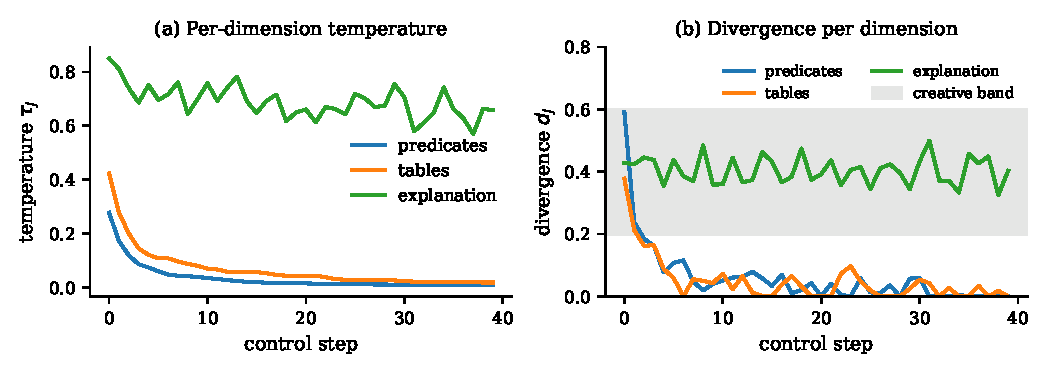
\includegraphics[width=\textwidth]{figures/fig5_selective_chaos.pdf}
\caption{E5. Per-dimension temperature feedback: precision dimensions are driven to low divergence while the creative dimension stays inside its band.}
\label{fig:selective}
\end{figure}

\begin{figure}[t]
\centering
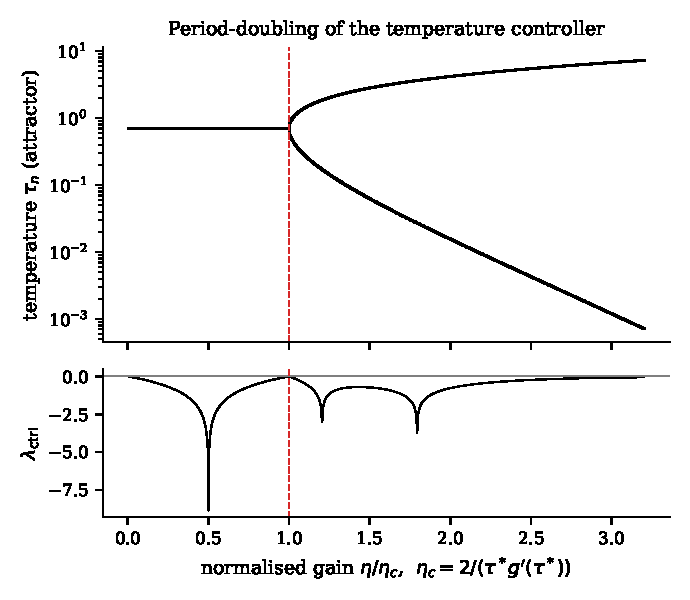
\includegraphics[width=0.62\textwidth]{figures/fig6_controller_bifurcation.pdf}
\caption{E6. Bifurcation diagram of the temperature law~\eqref{eq:temp} against normalised gain (top) and the controller's Lyapunov exponent (bottom). The dashed line marks the predicted $\eta_c$.}
\label{fig:bif}
\end{figure}

%% ===================================================================
\section{Applications beyond language models}
\label{sec:applications}

SCC requires only (i) a decomposition of a system's output or state into dimensions, (ii) a way to produce small perturbations or ensembles, and (iii) a set of cheap interventions. Several domains already have the first two.

\paragraph{Autonomous robots: creative exploration with safety controllers}
A robot that acts on its own faces a multi-dimensional decision: route, strategy and manner of approach, but also speed, force, distance to people and rule compliance. SCC assigns the first group a creative role and lets controlled chaos generate diverse candidate behaviours; the second group receives precision controllers that intervene, for instance by vetoing or projecting the action, whenever their divergence or a safety margin leaves its band, and the master controller composes an action only from admissible dimensions. This realises chaotic but safe exploration. A precedent is the hexapod robot of Steingrube et al.~\cite{steingrube2010}, whose small neural circuit switches gaits through chaos control and escapes traps by briefly releasing chaos. SCC generalises that idea from one oscillator to many semantic decision dimensions and adds a predictability horizon for re-planning.

\paragraph{Human cognition and neural signals}
Brain activity has long been analysed as chaotic. Freeman's olfactory model places perception on chaotic attractors~\cite{skarda1987}, early EEG studies estimated Lyapunov exponents across the sleep cycle~\cite{babloyantz1985}, and reviews discuss both the evidence and the methodological caveats~\cite{korn2003,stam2005}, as well as metastable coordination between brain regions~\cite{tognoli2014}. Per-channel short-term Lyapunov exponents with threshold-triggered warnings have been used for seizure prediction~\cite{iasemidis2003}, a direct precedent for a chaos map with selective alarms. SCC's dimension-wise exponent and horizon offer a common vocabulary to report which components of a cognitive or physiological signal are stable, which are wandering, and how far ahead each is predictable.

\paragraph{Crime-pattern predictability}
Aggregate crime exhibits self-exciting dynamics~\cite{mohler2011}, nonlinear hotspot formation~\cite{short2008}, and entropy scaling consistent with low-dimensional chaos~\cite{melgarejo2018}. A dimension-wise analysis, separating time of day, location, offence type and season, would report \emph{how predictable} each component of a pattern is and for how long, rather than a single forecast. We restrict this to aggregate, area-level patterns. Predictive policing trained on biased records can reproduce the bias~\cite{lum2016} and create runaway feedback loops~\cite{ensign2018}; the minimal-intervention principle and explicit horizon reporting are intended to discourage over-confident long-range use, and the framework is not intended for profiling individuals.

\paragraph{Human activity and mobility tracking}
Human mobility has an entropy-based predictability ceiling of about $93\%$~\cite{song2010}, and local divergence exponents of individual gait variables distinguish normal from pathological walking~\cite{dingwell2000,bruijn2013}. For wearable activity recognition~\cite{wang2019har}, per-dimension exponents over learned feature channels, together with the agent Lyapunov time, give a principled schedule for re-calibration and for deciding which activity components can be forecast and over what horizon.

%% ===================================================================
\section{Empirical evaluation protocol}
\label{sec:protocol}
The accompanying implementation runs SCC against any chat-completion interface. The planned evaluation uses the Spider and BIRD development sets~\cite{yu2018spider,li2023bird}, scored by execution accuracy, with:
\begin{itemize}
\item \emph{Baselines}: single greedy decoding; self-consistency by execution-result voting~\cite{wang2023sc}; verify-all, which regenerates every dimension with grounding; and decomposed pipelines~\cite{pourreza2023}.
\item \emph{Ablations}: no perturbation (sampling noise only); a scalar divergence in place of the dimension-wise exponent; a global temperature in place of the per-dimension law; and a fixed checkpoint interval in place of the horizon schedule.
\item \emph{Metrics}: execution accuracy; calls and tokens per question; the localisation AUROC of $\hat\lambda_j$ against per-dimension correctness, obtained by decomposing the gold query; and the calibration of the bracket~\eqref{eq:bracket}.
\item \emph{Multi-step agents}: success against checkpoint budget on multi-turn database tasks such as Spider~2.0~\cite{lei2025spider2}, comparing fixed and Lyapunov-time schedules.
\end{itemize}

%% ===================================================================
\section{Discussion and limitations}
\label{sec:discussion}
SCC treats an LLM agent the way chaos control treats a nonlinear oscillator: measure where perturbations grow, intervene minimally and only there, and plan around a finite predictability horizon. Its strongest guarantees (Propositions~\ref{prop:bracket},~\ref{prop:temp} and~\ref{prop:horizon}) are model-free, while Proposition~\ref{prop:joint} assumes independence across dimensions; correlated errors weaken the factorised advantage, and the consistency repair in the master controller is designed for that case. The quantitative results of Section~\ref{sec:numerics} are synthetic; their size on real models must be established by the protocol of Section~\ref{sec:protocol}. The method needs a semantic decomposition, which is straightforward for structured outputs (SQL, code, plans, robot actions) but requires learned or rubric-based parsers for free text. The finite-step exponent depends on the perturbation family and on $K$: the divergence for $K=5$ takes few distinct values, and larger ensembles or continuous metrics give finer resolution. Finally, SCC uses the vocabulary of dynamical systems at the level of observable outputs; connecting the output-level chaos map to internal Lyapunov spectra~\cite{engelken2023,li2025quasi} and to activation steering as a control input~\cite{li2023iti} is an open direction.

%% ===================================================================
\section{Conclusion}
\label{sec:conclusion}
Chaos theory explains why long-range forecasts fail and how sensitive systems can be steered cheaply. We carried both lessons into LLM agents by measuring instability per output dimension, intervening only where it is harmful, preserving it where it is creative, and scheduling re-anchoring by an agent Lyapunov time. The theory links observed divergence to error, shows why factorised control beats joint voting, and characterises the stability and period-doubling of the controller. The simulations show error localisation, better accuracy at lower cost, and markedly more reliable long-horizon agents. The same principles apply to autonomous robots and to neural, behavioural and social time series, wherever a system should be stable in some dimensions and free in others.

%% ===================================================================
\section*{CRediT authorship contribution statement}
\textbf{Kuhan K:} Conceptualization, Methodology, Software, Formal analysis, Investigation, Visualization, Writing -- original draft, Writing -- review \& editing.

\section*{Declaration of competing interest}
The author declares that he has no known competing financial interests or personal relationships that could have appeared to influence the work reported in this paper.

\section*{Data availability}
No external data were used. The simulation code, framework implementation and evaluation scripts are available from the author on reasonable request and will be deposited in a public repository upon publication.

\section*{Funding}
This research did not receive any specific grant from funding agencies in the public, commercial, or not-for-profit sectors.

\section*{Declaration of generative AI and AI-assisted technologies in the manuscript preparation process}
\textcolor{red}{[To be completed by the author before submission, in accordance with the journal's policy.]}

\bibliographystyle{elsarticle-num}
\bibliography{references}

\end{document}
